\documentclass[a4paper,12pt]{article}
\usepackage[utf8]{inputenc}
\usepackage{titlesec}
\usepackage{xcolor}
\usepackage{graphicx}
\usepackage{fancyvrb}

\usepackage[paperwidth=595pt,paperheight=841pt,top=56pt,right=56pt,bottom=56pt,left=56pt]{geometry}

%opening
\title{Attendance System Using Face Recognition}
\author{Kunal Mehta, Syed Mohammed Yousuff Hussain}
\titleformat{\section}{\Large\bfseries\filcenter}{\thesection}{0.5em}{}

\begin{document}
\tableofcontents
\maketitle

\begin{abstract}
This project is a part of e-Yantra Summer Internship program, 2015. The project is undertaken by Syed Yousuff and Kunal Mehta 
under the guidance of Mr.Viral and Mr.Yamik Mangukia. The end goal of this project is to build an automatic logging system 
using image processing for face recognition. The cameras placed at the entrance and exit of the lab will capture the image of 
a person entering or leaving the lab. Facial recognition on the images will be applied and the identity of the person will be 
extracted from the images. Sensors to determine the height of the person are placed near the entry and the exit. The height data
aids the facial recognition and improves the accuracy of the system. The recognition data will be automatically logged. The 
system will also include a GUI application that will monitor the system and also help in viewing the logs.
\end{abstract}

\newpage

\section{Getting Started}
\subsection{Introduction}
This project involves the use of various tools of image processing to recognize faces and develop an efficient attendance recording
system. Opencv library is used with Python to develop the project on Ubuntu platform. 

\subsection{Tools used}

 \subsubsection*{Opencv}
 Opencv is a powerful and platform independent library for Computer vision related applications spanning very basic tasks like pre-image 
 processing, color conversions to high level algorithms like feature extraction, machine learning etc. It is a free software and provides
 a rich Application Programming Interface for C, C++ and Python.

 \subsubsection*{Numpy}
 Numpy is a fundamental package for scientific computing with Python. Most important use of numpy for this project is that it contains
 a powerful N-dimensional array objects. We use 2 dimensional arrays provided by numpy to hold image data.

 \subsubsection*{Python}
 Python is used to write all the programs and it uses the installed opencv and numpy packages.

 \subsubsection*{Matplotlib}
 Matplotlib is a python 2D plotting library which produces publication quality figures in a variety of hardcopy formats and interactive 
 environments across platforms.

 \subsubsection*{IDLE}
 IDLE is an integrated development environment for Python.
 
 \subsubsection*{Arduino}
 The Arduino IDE was used to program the Arduino Mega development kit. This   kit was used to interface the ultrasonic distance measuring 
 sensor in order to use the height of the subjects to aid the face recognition and to increase accuracy. Considerable improvements were 
 noticed after adding height measurement to the system.


\subsection{Installation and setup}

\subsubsection*{Installing Opencv}
\begin{itemize}
 \item Download the opencv\textunderscore latest$\cdot$sh script file from the github repository. The link is given below
 \newline \textcolor{purple}{https://github.com/jayrambhia/Install-OpenCV/tree/master/Ubuntu}
 
 \item Save the file as opencv$\cdot$sh
 
 \item Navigate to the directory containing this file and change the permissions of the file and give it execution permission
 \newline \textcolor{blue}{chmod +x opencv.sh}
 
 \item Run the script file
 \newline \textcolor{blue}{./opencv.sh}
 \end{itemize}

\subsubsection*{Installing Numpy}
\begin{itemize}
 \item Run the command 
  \newline \textcolor{blue}{sudo apt-get install python-numpy}
\end{itemize}

\subsubsection*{Installing Matplotlib}
\begin{itemize}
 \item Run the command
  \newline \textcolor{blue}{sudo apt-get install python-matplotlib}
\end{itemize}

\subsubsection*{Installing IDLE}
\begin{itemize}
 \item Run the command
   \newline \textcolor{blue}{sudo apt-get install IDLE}
\end{itemize}

\subsubsection*{Installing Arduino}
\begin{itemize}
 \item Arduino IDE can be most easily installed from the Ubuntu software centre or can also be installed using the following command.
  \newline \textcolor{blue}{sudo apt-get install arduino}
\end{itemize}

\newpage
\section{Basic image operations}
\subsection{Introduction}
This section deals with basic image operations like reading an image from a file, performing different operations on images and 
saving back images to a file. Towards the end of this section, details are given as to how the inbuilt webcam or an external 
camera can be used to capture images and videos using Opencv and Python.

\subsection{Bare Minimum}
To perform almost any of the image operations discussed below, the \emph{cv2} and the \emph{numpy} libraries need to be imported.
\begin{itemize}
 \item To use this function, the \emph{ cv2} and \emph{numpy} libraries need to be imported.
 \newline \textcolor{blue}{import cv2}
 \newline \textcolor{blue}{import numpy}
\end{itemize}

\subsection{Reading image from a file}
\begin{itemize}
 \item Images can be read into a numpy array using the following line of code
 \newline \textcolor{blue}{Image\textunderscore name = cv2.imread('image\textunderscore name\textunderscore with\textunderscore location’)}
 \item The \emph {Image\textunderscore name} is a user defined variable that refers to the numpy array corresponding to the image.
 
\end{itemize}

\subsection{Writing image to a file / Saving an image}
\begin{itemize}
 \item Images can be saved to a file using the following line of code
 \newline \textcolor{blue}{cv2.imwrite(‘name\textunderscore to\textunderscore save\textunderscore with’, image\textunderscore name)}
 \item \emph{name\textunderscore to\textunderscore save\textunderscore with} is the name of the image with the location at which the image
 needs to be stored. 
 \item \emph{image\textunderscore name} is the name of the np array corresponding to the image.
 
\end{itemize}

\subsection{Displaying an image to the screen}
\begin{itemize}
 \item Images can be displayed using the following line of code:
 \newline \textcolor{blue}{ cv2.imshow(“window\textunderscore name”, image\textunderscore name)}
 \item A window is created with the name \emph{window\textunderscore name} and the image corresponding to the numpy array
 \emph{image\textunderscore name} is  displayed on the window.
 
\end{itemize}

\subsection{Converting between Color formats}
\begin{itemize}
 \item Images can be easily converted between one color format to the other using the following line of code.
 \newline \textcolor{blue} {cv2.cvtcolor(image\textunderscore name, color\textunderscore format\textunderscore 1 2  color\textunderscore format\textunderscore 2)}
 \item \emph{color\textunderscore format\textunderscore 1} is the original color format of the image.
 \item \emph{color\textunderscore format\textunderscore 2} is the desired color format for the image.
 \item One example of the color format conversion that converts the image from BGR color format to the gray color format is given below
 \newline \textcolor{blue}{cv2.cvtcolor(Image\textunderscore name, BGR2GRAY)}
 \end{itemize}

\subsection{Cropping images / Region of Interest}
\begin{itemize}
 \item Images can be easily cropped in opencv. Since images are represented as numpy arrays in opencv, selecting only a specific
 number of rows and columns from one numpy array and assigning it to a new array. 
 \item To obtain the number of rows and columns in an image, the following function can be used.
 \newline \textcolor{blue}{image\textunderscore name$\cdot$shape}
 \item \emph{image\textunderscore name} is the name of the numpy array corresponding to the image.
 \item This function returns the shape of the image, i,e the number of rows and columns present in the image. It also returns 
 the third dimension of the array in case of colored images.
 \item The specific rows and columns can be selected from this image and assigned to the new image. For example, if the top half
 of the image is to be cropped, then the following lines of code can be used.
 \newline \textcolor{blue}{rows, colummns, colors = image\textunderscore name$\cdot$shape}
 \newline \textcolor{blue}{new\textunderscore image = image\textunderscore name[rows/2, columns, :]}
\end{itemize}
 
\subsection{Resizing images}
\begin{itemize}
 \item Images can be resized using the following line of code
 \newline \textcolor{blue}{new\textunderscore image = cv2.resize(image\textunderscore name, (width, height), interpolation = cv2.INTER\textunderscore CUBIC)}
 \item Here, width is the desired width of the final\textunderscore image and height is the desired height of the image. 
 \item Interpolation refers to the technique that is employed to calculate the values of pixels that are newly added or 
  to select the pixels that are to be removed.
 \item Different interpolation techniques can be used to resize images. More details can be found from the Opencv documentation. 
 \end{itemize}

\subsection{Working with videos}
\begin{itemize}
 \item The webcam is used in most of the real time applications. To do so, the \emph{VideoCapture} object can be used. Using
 this object, either a video file can be read frame by frame or a webcam can be opened and frames can be read into the program.
 \item The following line of code is used to create a VideoCapture object-
 \newline \textcolor{blue}{object\textunderscore name = cv2$\cdot$VideoCapture(index)}
 \item To open the inbuilt webcam, set index = 0.
 \item To use an external camera, use the index = 1, 2, 3 and so on in increasing order.
 \item To read from a video file, use the file location as the index.
 \item To capture a frame using the \emph{VideoCapture} object, use the following line of code
 \newline \textcolor{blue}{return, frame = object\textunderscore name$\cdot$read(0)}
 \item The return value is true if the frame is successfully read. Else, it is 0.
 \item The frame is read in as a numpy array.
 \item The resuorce opened by the VideoCapture object has to be released once its use is over. The below line of code can be used.
 \newline \textcolor{blue}{object\textunderscore name$\cdot$release()}
\end{itemize}

\newpage
\section{Contours}
\subsection{Introduction}
Contours are, in simple, curves joining all the continuous points (along the boundary), having same color or intensity. Contours 
are a useful tool for shape analysis and object detection and recognition. For better accuracy, use binary images. So before finding
contours, apply threshold. FindContours function provided by the opencv library modifies the source image. So if you want source image
even after finding contours, store it to some other variables. The following line of code illustrates the use of the findContours 
function provided by the opencv library
\vspace{1cm}

\textcolor{blue}{output\textunderscore image, contours, hierarchy = cv2$\cdot$findContours(INPUT\textunderscore IMAGE,
					cv2$\cdot$RETR\textunderscore TREE,
					cv2$\cdot$CHAIN\textunderscore APPROX\textunderscore SIMPLE)}

\vspace{1cm}
Here, \emph{output\textunderscore image} is the final image, \emph{contours} is a list of contours present in the \emph{input\textunderscore image}.
\emph{contour} is a numpy array of (x,y) coordinates of boundary points of the object. The first argument is the input image, the second 
argument is the contour retrieval mode and the third argument is the chain approximation method. The simple chain approximation is useful 
when the image contains rectangular contours. In such cases, only the endpoints or vertices of the rectangular are sufficient to denote the
contour instead of storing all the points on the rectangle. This saves memory space.s
			
\subsection{Drawing Contours}
The list of contours returned by the function contains all the contours identified in the image by the function. The contours are labeled with 0 based indices. 
All contours can be drawn or a specific contour can be drawn based on the requirement.
\vspace{0.5cm}
\newline To draw all the contours in an image:
\newline \textcolor{blue}{image = cv2$\cdot$drawContours(image, contours, -1, (0,255,0), 3)}
\vspace{0.5cm}
\newline To draw an individual contour, say 4th contour:
\newline \textcolor{blue}{image = cv2$\cdot$drawContours(image, contours, 3, (0,255,0), 3)}
\vspace{0.5cm}
\newline The fourth argument specifies the color to be used to draw the contours and the fifth argument specifies the thickness
of the contour to be drawn.

\subsection{Contour approximation method}
This is the third argument to the function. As contours are the boundaries of a shape with same intensity, 
it stores the (x,y) coordinates of the boundary of a shape. But does it store all the coordinates ? That is specified by this contour 
approximation method.
\vspace{0.5cm}
\newline If \textcolor{blue}{cv2$\cdot$CHAIN\textunderscore APPROX\textunderscore NONE} is passed, all the boundary points are stored. But actually do we need all the points? For egg, 
if contour is a straight line, then we do not need all the points on the line to represent that line. We need just two end points 
of that line.This is what \textcolor{blue}{cv2$\cdot$CHAIN\textunderscore APPROX\textunderscore SIMPLE} does. It removes all redundant points and compresses the contour, thereby saving memory.
\vspace{0.5cm}
\newline
Our project did not require the use of contours but still we studied contours as it is a versatile topic in image processing. It
is recommended that more reading should be done on contours from the opencv documentation.

\newpage
\section{Detection of Different Objects using Open CV-Python}

\subsection{Introduction}
Object detection is a computer technology related to computer vision and image
processing that deals with detecting instances of semantic objects of a certain
class (such as humans, buildings, or cars) in digital images and videos.
Well-researched domains of object detection include face detection and pedestrian
detection. Object detection has applications in many areas of computer vision,
including image retrieval and video surveillance. We basically started with
detection of skin, face, eye and then moved towards detectign objects like cars and bottles.
More details can be found here-
\newline \textcolor{purple}{http://docs.opencv.org/modules/ocl/doc/object\_detection.html}

\subsection{Skin Detection}

Skin detection is the process of finding skin-colored pixels and regions in an image or a
video. This process is typically used as a pre-processing step to find regions that potentially 
have human faces and limbs in images. Several computer vision approaches have been developed for skin detection. 
The skin detectors transform the given pixel into an appropriate color space and then use a skin classifier 
to label the pixel whether it is a skin or a non-skin pixel. A skin classifier defines a decision boundary of 
the skin color class in the color space based on a training database of skin-colored pixels.

Skin color and textures are important cues that people use consciously or unconsciously to infer variety of culture-related 
aspects about each other. Skin color and texture can be an indication of race, health, age, wealth, beauty, etc. 
However, such interpretations vary across cultures and across the history. In images and videos, skin color is an indication of 
the existence of humans in such media. Skin detection means detecting image pixels and regions that contain skin-tone color.


A Framework for Skin Detection Skin detection process has two phases: a training phase and a detection phase. 
Training a skin detector involves three basic steps: 

\begin{itemize}
 \item Collecting a database of skin patches from different images. Such a database typically contains skin-colored patches from a 
  variety of people under different illumination conditions.
 \item Choosing a suitable color space.
 \item Learning the parameters of a skin classifier.Given a trained skin detector, identifying skin pixels in a given image or 
  video frame involves: 
  \begin{itemize}
    \item	Converting the image into the same color space that was used in the training phase. 
    \item	Classifying each pixel using the skin classifier to either a skin or non-skin. 
    \item	Typically post processing is needed using morphology to impose spatial homogeneity on the detected regions.
  \end{itemize}
\end{itemize} 

\begin{center}
	\graphicspath{ {images/} }
	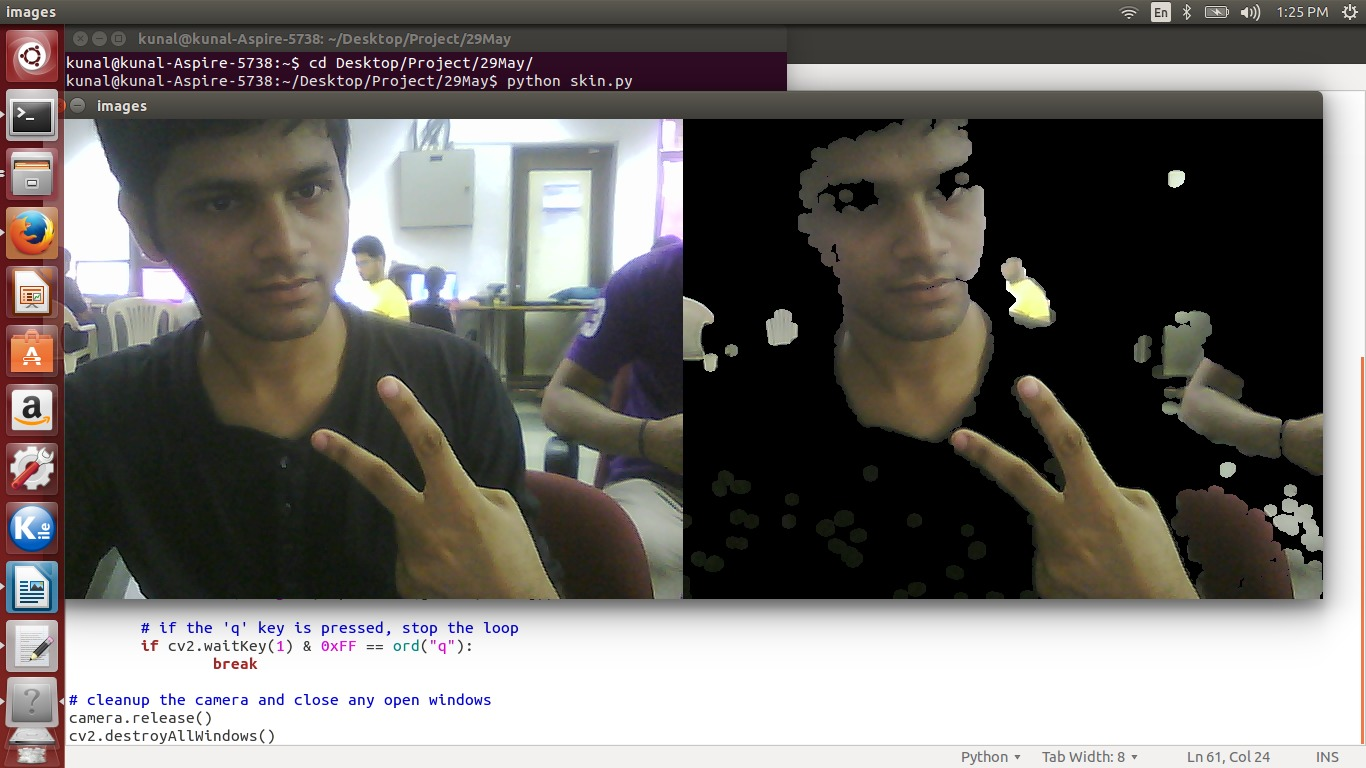
\includegraphics[width=15cm, height=7.5cm]{skin}
\end{center}

For More details, watch:
\newline
\textcolor{purple}{https://www.youtube.com/watch?v=HbqG1By2kas}

\subsection{Face \& Eye Detection using Haar-based cascade classifiers}

Object Detection using Haar feature-based cascade classifiers is an effective object detection method proposed by Paul Viola 
and Michael Jones in their paper, "Rapid Object Detection, using a Boosted Cascade of Simple Features" in 2001. It is a machine 
learning based approach where a cascade function is trained from a lot of positive and negative images. It is then used to detect 
objects in other images. In this process, we basically need a lot of database of images. A database consisting if positive images 
(facial images) and another database of negative images (non-facial images). These databases are required specifically for training 
the classifier. The classification is a binary one (consist of two classes 1 (face) \& 0 (non-face). After classifying it into two 
classes, we need to extract features from it. For this, Open CV provides lots of Haar features like edge, line, four-rectangle, etc. 
They basically go through the entire image, basically the matrix consisting of image pixels for the process of convolution. 
However, there are large numbers of features that are extracted. Using all the features will just eat up the processing time and memory.
So, extra, unrequired features are eliminated using Adaboost technique.Now taking an image and applying all the necessary features 
on it to identify the facial position will just increase the time. To avoid this, features are applied one-by one after classifying 
them into groups of classifiers. This is called cascade classifying.OpenCV already contains many pre-trained classifiers for face, 
eyes, smile etc. Those XML files are stored in opencv/data/haarcascades/ folder. Let's create face and eye detector with OpenCV.


For more information:

\textcolor{purple}{http://docs.opencv.org/master/d7/d8b/tutorial\_py\_face\_detection.html}

\textcolor{purple}{https://realpython.com/blog/python/face-detection-in-python-using-a-webcam/}

\subsection{Car Detection (Training our own classifiers)}

  All the above based detection methods can be used for detecting different objects such as cars, etc. Here the same step follows 
except for the place where we were using already available cascade classifier file, here we will create our own cascade classifier.
There are two applications in OpenCV to train cascade classifier: 

\begin{enumerate}
	\item 	opencv\_haartraining 
	\item 	opencv\_traincascade.
\end{enumerate}

The main difference between the two applications is that opencv\_traincascade supports both Haar and LBP (Local Binary Patterns) 
features. LBP features are integer in contrast to Haar features, so both training and detection with LBP are several times faster 
than that with Haar features. Regarding the LBP and Haar detection quality, it depends on training: the quality of training dataset 
first of all and training parameters too. It’s possible to train a LBP-based classifier that will provide almost the same quality as 
Haar-based one. Also there are some auxiliary utilities related to the training.opencv\_createsamples is used to prepare a training 
dataset of positive and test samples. opencv\_createsamples produces dataset of positive samples in a format that is supported by both 
opencv\_haartraining and opencv\_traincascade applications. The output is a file with *.vec extension, it is a binary format which 
contains images. opencv\_performance may be used to evaluate the quality of classifiers, but for trained by opencv\_haartraining only. 
It takes a collection of marked up images, runs the classifier and reports the performance, i.e. number of found objects, number of
missed objects, number of false 
alarms and other information.

\begin{center}
	\graphicspath{ {images/} }
	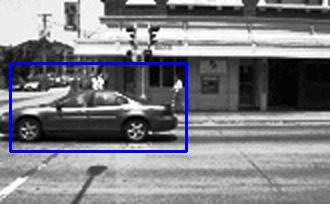
\includegraphics[width=12cm, height=6cm]{car}
\end{center}

For car detection, we took almost 550 positive (car) images \& 500 negative (non-car) images. The first step was to classify. 
It included creating an .info file containing information about the location, size, no. of cars in each of the positive image. 
We also created .txt file containing location of negative images. opencv\_traincascade was used to train the samples. Initially, 
6 stages were used (1 input, 1 output \& 4 hidden layer). However the accuracy was less. Later, 18 stages were used (of course, 
with different weights). This increased the accuracy of the detection. The images used for training are called training data sets 
while that for checking the output are called testing data set.

\begin{center}
	\graphicspath{ {images/} }
	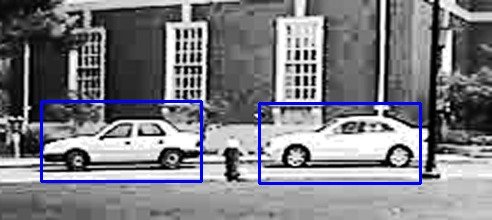
\includegraphics[width=12cm, height=6cm]{car1}
\end{center}

\subsection{Bottle Detection}
The same process as that for car detection was used to detect soft drinks bottles like pepsi, coco-cola, Tupperware, mirinda, etc. 
However the accuracy was much less since we used only 20 positive images for training.

\begin{center}
	\graphicspath{ {images/} }
	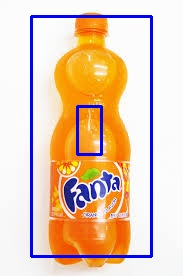
\includegraphics[width=7cm, height=10cm]{bottle_detected}
\end{center}

\newpage
\section{Face Recognition}
\subsection{Introduction}
This particular task was performed as part of e-Yantra Summer Internship program, 2015. The task is to recognize a face. 
The complete program can be found at the git hub repository in the links given at the end of the document. The program takes 
the test image as a command line argument and returns the label corresponding to the given face and the level of confidence of 
detection. Note that the underlying theory and the working of the underlying algorithms involved in the face recognition process 
are not discussed. The functions provided by Opencv are directly used. For more details regarding the underlying algorithms, 
visit the links given in the reference section. The work of Bikramjot Singh Hanzra has been heavily used from his blog, 
“face recognition using python and opencv” thoughout the task. 

The whole process can be divided in three major steps -
\begin{enumerate}
 \item The first step is to find a good database of faces with multiple images for each induvidual. 
 \item The next step is to detect faces in the database images and use them to train the face recognizer. 
 \item The last step is to test the face recognizer to recognize faces it was trained for.
\end{enumerate}

\subsection{Face Database}
We used Yale face database available for download from this link
\\
\newline \textcolor{purple}{http://vision.ucsd.edu/content/yale-face-database}
\\
\\
It contains 165 grayscale images of 15 individuals in gif format, There are 11 images for each individual.
In each image, the individual has a different facial expression like happy, sad, normal, surprised, sleepy etc.
Indeed, there are 166 images with 12 images for the first individual.

We used this database by using 10 images of the total 11 images of each individual in training our face recognizer and the 
remaining single image of each individual to test our face recognition algorithm.
The images corresponding to each individual are named like subject number. facial\textunderscore expression where number ranges 
from 01, 02, 03…, 14, 15 and facial\textunderscore expression is the expression that the individual has in the image. We did not use the 
image with .sad extension for training and used it for testing.

\subsection{Detecting faces and training the recognizer}
The first step is to detect the face in each image. Once, we get the region of interest containing the face in the image, 
we will use it for training the recognizer. For the purpose of face detection, we will use the Haar Cascade provided by OpenCV. 
The haar cascades that come with OpenCV are located in the /data/haarcascades> directory of your OpenCV installation.
We will use haarcascade\textunderscore frontalface\textunderscore default.xml for detecting the face. So, we load the cascade using the cv2.CascadeClassifier 
function which takes the path to the cascade xml file.
\\
\newline \textcolor{purple}{face\textunderscore cascade = cv2.CascadeClassifier('haarcascade\textunderscore frontalface\textunderscore default.xml')}
\\
\\
Once the face detector is ready, we will use it to detect the faces from the database. These faces were added to a list and 
labels corresponding the face were added in a separate list. All faces of an indivisual were assigned the same label. To do this, 
a function is written get\textunderscore training\textunderscore set, which does the following:

\begin{enumerate}
 \item Take input, the path of the folder containing the images.
 \item Detect the faces from the database and add them to the list as separate images. Here, all faces but the ones 
 with $\cdot$sad extension are added. .sad extension images are used as a testing set. So, it is not included in the training set.
 \item Extract the label from the image name and add it to a separate list 
 \item Return both the lists to the calling program
\end{enumerate}

\begin{verbatim}
def get_training_set(path): 
    image_paths = [ os.path.join(path, f) for f in os.listdir(path) if not f.endswith('.sad')] 
    images = [ ]
    labels = [ ] 
    for image_path in image_paths: 
    image_pil = Image.open(image_path).convert('L') 
    image = np.array(image_pil, 'uint8') 
    label = int(os.path.split(image_path)[1].split(".")[0].replace("subject", "")) 
    faces = face_cascade.detectMultiScale(image) 
    for (x, y, w, h) in faces: 
    images.append(image[ y: y + h, x: x + w] ) 
    labels.append(label) 
    return images, labels 
\end{verbatim}

Once the training set (the list of images and the list of labels) was ready, the recognizer was trained. Opencv provides 3 face recognizers:

\begin{enumerate}
 \item Eigenface face recognizer : \textcolor{blue}{createEigenFaceRecognizer()}
 \item Fisherface face recognizer : \textcolor{blue}{createFisherFaceRecoginzer()}
 \item Local Binary Pattern Histogram face recognizer : \textcolor{blue}{createLBPHFaceRecoginzer()}
\end{enumerate}

We used LBPH face recognizer for the task of face recognition.
\\
\newline \textcolor{blue}{face\textunderscore recognizer = cv2.createLBPHFaceRecognizer()}
\\
\\
The next task is to train the recognizer with the training set. We use the above defined function get\textunderscore training\textunderscore set to get 
the training set from the database. 
\\
\newline \textcolor{blue}{images, labels = get\textunderscore training\textunderscore set('./yalefaces/yalefaces') }
\\
\\
Then, by using this training set, we train the recognizer. 
\\
\newline \textcolor{blue}{face\textunderscore recognizer.train(images, np.array(labels))} 
\\
\\
\subsection{Testing the recognizer to recognize faces}
The trained recognizer is now tested using the test images. (images with .sad extension). 
\\
\newline \textcolor{blue}{labelDetected, confidence = face\textunderscore recognizer.predict(input\textunderscore image)}
\\
\\
labelDetected is the label corresponding to the detected image in the database. Confidence is the parameter specifying the 
accuracy level of the recognizer. A confidence level of 0 indicates that the face is recognized with 100% accuracy. 

The input\textunderscore image corresponds to only the face region of the image. This region can be extracted using the face\textunderscore cascade declared earlier. 

\subsection{Personal notes}
The above method was applied to a different database. 16 Images of Amir Khan were collected from the internet and a recognizer was 
trained to identify Amir khan's face. While testing the recognizer, the results were far less satisfactory since in most of the
images in the database, the person was not looking into the camera and the alignment of the face and the position of eyes and mouth 
in all the images were not uniform. Also, the training set of images did not contain a wide range of emotions and majority of the 
images were of uniform emotions. (you can guess it! His old smiling face). So, the confidence level of detection was always above 150. 

\newpage
\section{Integrating Height of a Person with LBPH based Facial Recognition.}

\subsection{Introduction}
now, we have  a handful experience with face recognition in OpenCV Python environment.We observed that accuracy of
face detection is not highly reliable and it might make mistakes in detection and recognition of  faces. This problem 
can be solved by integrating the height concept with the face recognition algorithm. We used Arduino and an Ultrasonic distance
sensor to measure the height of the person and used this data to improve the accuracy of the system.


\subsection{Arduino:}
Arduino is an open-source platform used for building electronics projects. Arduino consists of both a physical programmable 
circuit board (often referred to as a microcontroller) and a piece of software or IDE (Integrated Development Environment) that 
runs on your computer, used to write and upload computer code to the physical board.

The Arduino platform has become quite popular with people just starting out with electronics, and for good reason. 
Unlike most previous programmable circuit boards, the Arduino does not need a separate piece of hardware (called a programmer) 
in order to load new code onto the board – you can simply use a USB cable. Additionally, the Arduino IDE uses a simplified version
of C++, making it easier to learn to program. Finally, Arduino provides a standard form factor that breaks out the functions of the 
micro-controller into a more accessible package.

\subsection{Arduino Mega (Atmega2560)}
There is variety of Ardrinos available in the market. We finalised on using
Aurdino Mega.

\graphicspath{ {images/} }
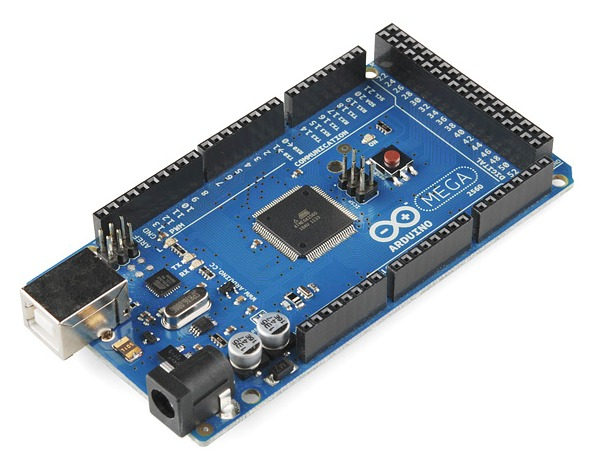
\includegraphics[width=300pt]{arduino}

The Arduino Mega is a microcontroller board based on the ATmega2560. It has 54 digital input/output pins (of which 14
can be used as PWM outputs), 16 analog inputs, 4 UARTs (hardware serial ports), a
16 MHz crystal oscillator, a USB connection, an ICSP header, and a
reset button. It contains everything needed to support the microcontroller;
simply connect it to a computer with a USB cable or power it with a DC source to get started. It even has an onboard voltage regulator.
The Mega is compatible with most shields designed for the Arduino Duemilanove or Diecimila.

The Mega 2560 R3 also adds SDA and SCL pins next to the AREF. In addition, there are two new pins placed near the RESET pin. 
One is the IOREF that allow the shields to adapt to the voltage provided from the board. The other is a not connected and is 
reserved for future purposes. The Mega 2560 R3 works with all existing shields but can adapt to new shields which use these 
additional pins.

\subsubsection*{Features}
\begin{enumerate}
	\item ATmega2560 microcontroller 
	\item Input voltage - 7-12V 
	\item 54 Digital I/O Pins (14 PWM outputs) 
	\item 16 Analog Inputs 
	\item 256k Flash Memory 
	\item  Clock Speed 16 MHz
\end{enumerate}

\subsubsection*{Setup}
We will walk you through downloading, installing, and testing the Arduino software 
(also known as the Arduino IDE - short for Integrated Development Environment).

All our work was done on a Linux machine running the Ubuntu flavor.
If you are a Linux user, you probably know that there are many different distribution ‘flavors’ of Linux out there. 
Unsurprisingly, installing Arduino is slightly different for many of these distributions. Luckily, the Arduino community 
has done an excellent job of providing instructions for most of the popular versions. Use the link below to learn more about installation
of Arduino IDE on your system.
\newline \textcolor{purple}{http://playground.arduino.cc/Learning/Linux}

\subsubsection*{Writing your first application}
After following the appropriate steps for your software install, we are now ready to test your first program with your Arduino board!

\begin{enumerate}
	\item Launch the Arduino application. This is what You will see:
	\newline 
	\\
	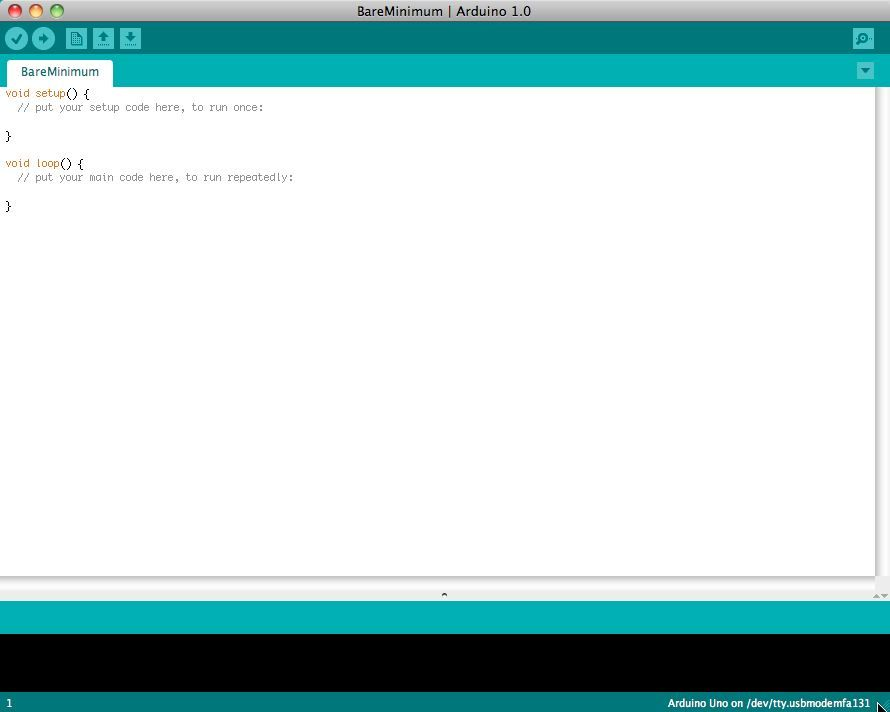
\includegraphics[width=200pt]{IDE}
	\item If you disconnected your board, plug it back in.
	\item open the Blink example sketch by going to: File $>$ Examples $>$ 1.Basics $>$ Blink
	\item Select the type of Arduino board you're using: Tools $>$ Board $>$ your board type
	\item Select the serial port that your Arduino is attached to: Tools $>$ Port $>$
xxxxxx (it’ll probably look something like “/dev/tty.usbmodemfd131” or “/dev/tty.usbserial-131” but probably with a different number) 
	\item	If you’re not sure which serial device is your Arduino, take a look at the available ports, then unplug your Arduino and look again. The one that disappeared is your Arduino
	\item With your Arduino board connected and the Blink sketch open, press the `Upload' button
	\item After a second, you should see some LEDs flashing on your Arduino(these are the RX and the TX LED's), followed by
the message `Done Uploading' in the status bar of the Blink sketch.
	\item If everything worked, the on board LED on your Arduino should now be blinking! You just programmed your first Arduino!
\end{enumerate}

\subsubsection*{Troubleshooting}
Arduino Playground Linux section is a great resource for figuring out any problems with your Arduino installation. It is common that
you may face some problems while uploading the code. Make sure that the USB cable is good. (We had problem uploading the code and we
tried a hundred different things to get it working but finally found that the problem was with the USB cable). Select the right port and 
the board from the tools menu. Make sure that the port selected is not in use by any other application.


\subsection{Ultrasonic Sensor}

\subsubsection*{Introduction}
HC-SR04 Ultrasonic Sensor is a very affordable proximity/distance sensor that has been used mainly for object 
avoidance in various robotics projects . It essentially gives your Arduino eyes / spacial awareness and can prevent your robot 
from crashing or falling off a table. It has also been used in turret applications, water level sensing, and even as a parking sensor. 
This simple project will use the HC-SR04 sensor with an Arduino and a Processing sketch to provide a neat little interactive display 
on your computer screen.

We used HC SR04 Ultrasonic module for height calculation. One can download the documentation from the official site:

\textcolor{purple}{http://www.micropik.com/PDF/HCSR04.pdf}

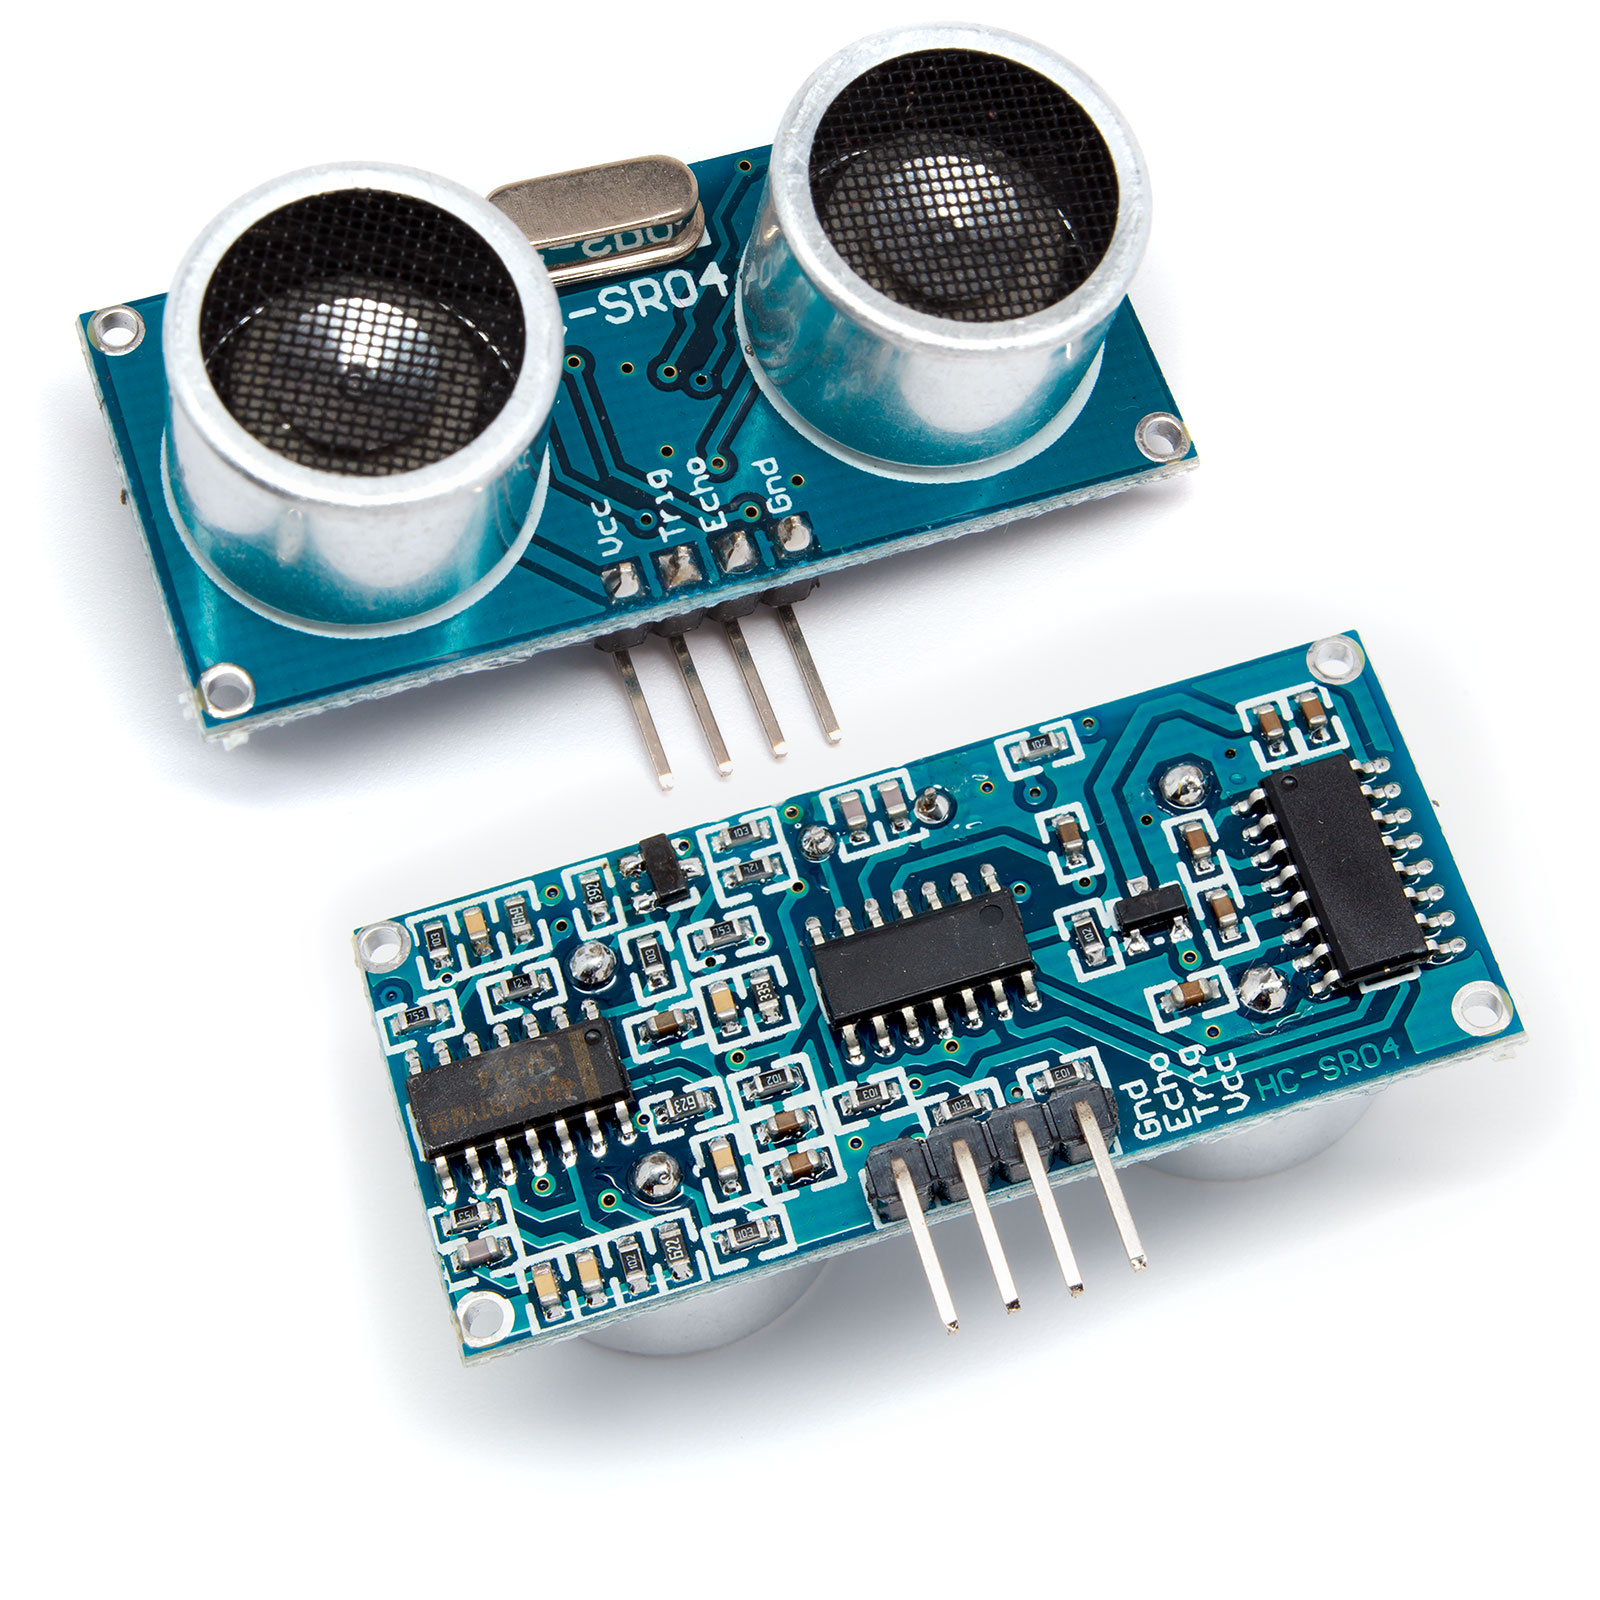
\includegraphics[width=300pt]{ultrasonic} 

\subsubsection*{Working of the sensor}
ULTRASONIC pulse travels with the speed of sound that is, 340$\cdot$29 m/s. An ultrasonic sensor like the one we used in our project consists
of an emitter and a receiver of ultrasonic sound waves. (Ultrasonic sound waves have a high frequency that humans cannot hear). The 
emitter emits ultrasonic sound waves. These sound waves travel in air, hit the object and reflect from its surface. The reflected 
waves are received by the receiver after some time. This time corresponds to the time the waves take to travel from the emitter to the 
object and from the object to the emitter after being reflected. 

The microcontroller (in our case, the Arduino) keeps track of this time, i, e, the time it takes for the receiver to receive after the 
emitter has sent out the waves. Knowing this time, the microcontroller is programmed to calculate the distance of the object since the 
speed of the waves is known. (340$\cdot$29 m/s). The simple formule \textcolor{blue}{distance = speed * time} is used.

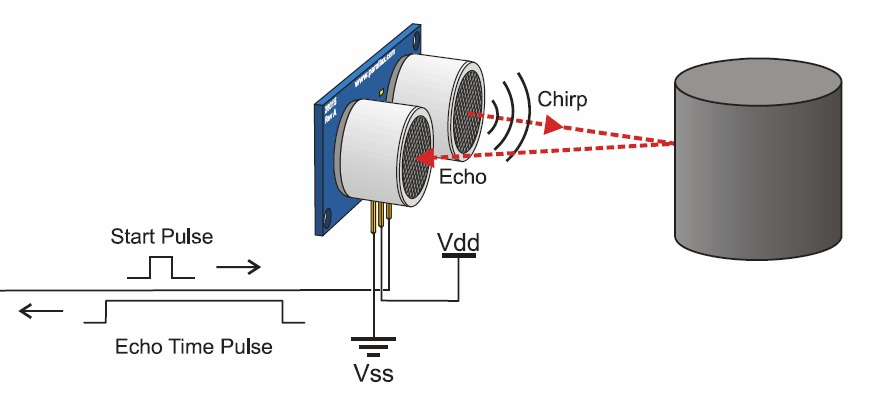
\includegraphics[width=240pt]{working}

\subsubsection*{Interfacing the sensor with the Arduino}
The sensor consists of 4 pins. The connections are listed below:

\begin{enumerate}
 \item Vcc------------------connect to 5V dc
 \item Trigger--------------pulse input that triggers the emitter. 
 \item Echo-----------------this pin indicates the reception of the echo.
 \item Gnd------------------ground
\end{enumerate}


The trigger pin and the echo pin can be connected to any of the GPIO pins of the Arduino. In our case, we conneced the trigger pin
to pin 8 and the echo pin to pin 7 of the Arduino. If you are using the code provided below, then make the same connections. Or you can
also redefine the trigPin and the echoPin according to the connections you make.
\\
\\
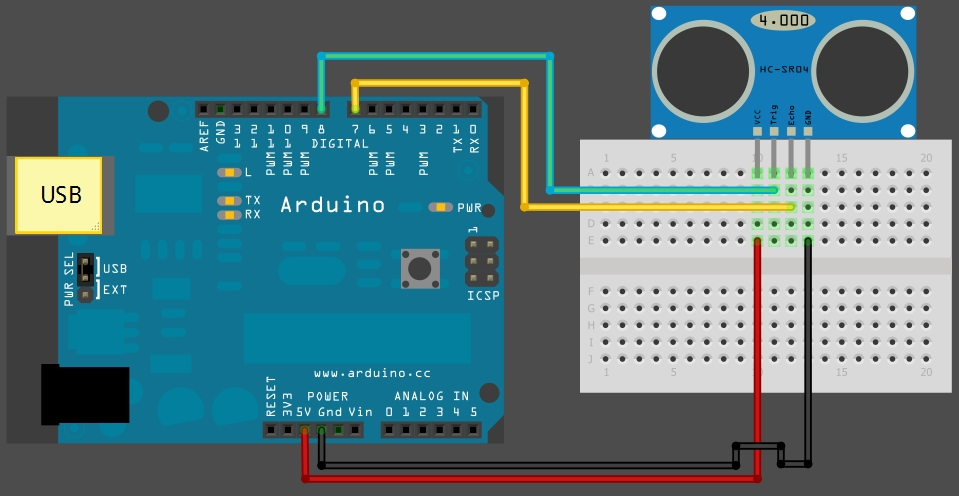
\includegraphics[width=300pt]{ardsketch}
\vspace{1cm}
\subsubsection*{Arduino code}
\begin{verbatim}
  #define trigPin 13
  #define echoPin 12

  void setup() {
    // put your setup code here, to run once:
    Serial.begin(9600);
    pinMode(trigPin, INPUT);
    pinMode(echoPin, OUTPUT); 
  }

  void loop() {
    // put your main code here, to run repeatedly:
  }

  int getDistance()
  {
    long duration;
    int distance;

    digitalWrite(trigPin, LOW);
    delayMicroseconds(2);
    digitalWrite(trigPin, HIGH);
    delayMicroseconds(10);
    digitalWrite(trigPin, LOW);

    duration = pulseIn(echoPin, HIGH);
    distance = (duration/2)/29.1;

    return distance;
  }

  void serialEvent() {
    if (Serial.available()) {
      char temp = Serial.read();
      if(temp == 's')
      {
          Serial.println(getDistance());
      }
    }
  }


\end{verbatim}


\newpage
\section{GUI and the final system assembly}
After Developing code for face detection and recognition and also an arduino code for height calculation, we moved to develop a 
final gui which can provide an easy interface and help view the results of recognition and the logs in an easy graphical wasy. 

Python Supports variety of libraries to design a GUI. After some research, we found the following best for 
designing GUI for our application

\subsection{Different options for creating GUI}
\subsubsection*{Kivy}
One of the more interesting projects, the liberal MIT-licensed Kivy is based on OPENGL CS 2 and includes native multi-touch for each 
platform and Android/iOS. It’s an event-driven framework based around a main loop, and is thus very suitable for game development 
Your application adds callbacks from the main loop at a scheduled frequency, or by one-off trigger. The Kivy framework is very powerful
for handling everything from widgets to animation, and includes its own language for describing user interface and interactions. 
If you want to create cross-platform graphical applications, or just need a very powerful cross-platform GUI, Kivy is highly 
recommended.

\subsubsection*{PyQt}
Qt is a multi-licensed cross-platform framework written in C++. If your application is completely open source, you can use Qt 
for free under the community license; otherwise you’ll need a commercial license. Qt has been around for a long time and was owned 
by Nokia for a while; it’s a very comprehensive library of tools and APIs, widely used in many industries, and covers many platforms 
including mobile. If a gadget such as a SatNav has a GUI, there’s a good chance it’ll be Qt based.
\newline We have used PyQt framework to run the GUI in our system.

\subsubsection*{PyGUI}
Compared to Kivy and PyQt, PyGUI is considerably simpler and just for Unix, Macintosh and Windows platforms. Developed 
by Dr. Greg Ewing at the University of Canterbury in New Zealand, the MVC framework focuses on fitting into the Python ecosystem
as easily as possible.
One of the platform’s aims is to interpose as little code as possible between the Python application and the platform’s 
underlying GUI so the application’s display always reflects the native GUI of the platform. If you’re after a simple and quick 
way to learn GUI, start with this one.

\subsubsection*{libavg}
This is another third-party library, written in C++ and scripted from Python, with properties of display elements as Python 
variables, a full-featured event handling system, timers (setTimeout, setInterval), support for logging and more. Like Kivy, libavg 
uses OpenGL and makes use of hardware acceleration.
Libavg runs on Linux, Mac OS X and Windows, and is open source and licensed under the LGPL. It’s been used extensively for 
artistic exhibitions and has a wide range of features such as a layout engine that can deal with thousands of objects 
(images, text, videos and camera output), fast video output, and a markup system for displaying text, as well as GPU shader
effects such as blur, Chromakery and more. Plugins written in C++ have access to all libavg internals.
If you ever see many people playing a multi-touch game on a large flat display, you might be looking at a good example of 
libavg in action.

\subsubsection*{wxPython}
There have already been two books written about wxPython, making it worth a mention even if it isn’t quite ready for Python 3.
WxPython is based on wxWidgets, a cross-platform GUI library written in C++. In addition to the standard dialogs, it includes a 
2D path drawing API, dockable windows, support for many file formats and both text-editing and word-processing widgets.
There’s a great set of demos provided with wxPython, along with several sets of tutorials to help get you started. Given that 
wxWidgets has a 22-year development pedigree, this is one of the most popular frameworks. Make sure you read the wikipedia.
This is a great set of frameworks that should cover most needs. However, we selected PyQt4, the latest version of PyQt for 
developing GUI for attendance System.

\subsection{Using PyQt}
Creating an application in PyQT4 may be done in a few ways. The most common one is to use QTDesigner, which we get with QT. 
QTDesigner is a drag and drop tool that lets us design the GUI which is very handy for complicated interfaces. We can place widgets on 
the window, add names etc. To create an application in PyQT4, the following steps need to be followed.


\begin{enumerate}
	\item Download the PyQt4 package. Use the following command:
	 \newline \textcolor{blue}{sudo apt-get install pyqt4-dev-tools}
	\item Download QTDesigner. This can be found on the Ubuntu software centre.
	\item Create the GUI in QTDesigner. This is just a drag and drop job.   
	\item Set proper names for each widget in the property editor.This is important to code easily.
	\item Save the design. The file will be saved as .ui file. If you open this file in an editor, you'll notice that is 
	 is just an xml file.
	\item Using pyuic4 create the python GUI class. Use the following command to do this:
	 \newline \textcolor{blue}{pyuic4 filename$\cdot$ui \textgreater  outputFileName$\cdot$py}
	\item Instanciate this GUI class and call the application from within this class.
	\item You will need to use a timer to update the GUI continuously as the application runs.
\end{enumerate}

The GUI we created looks like the one shown below. 

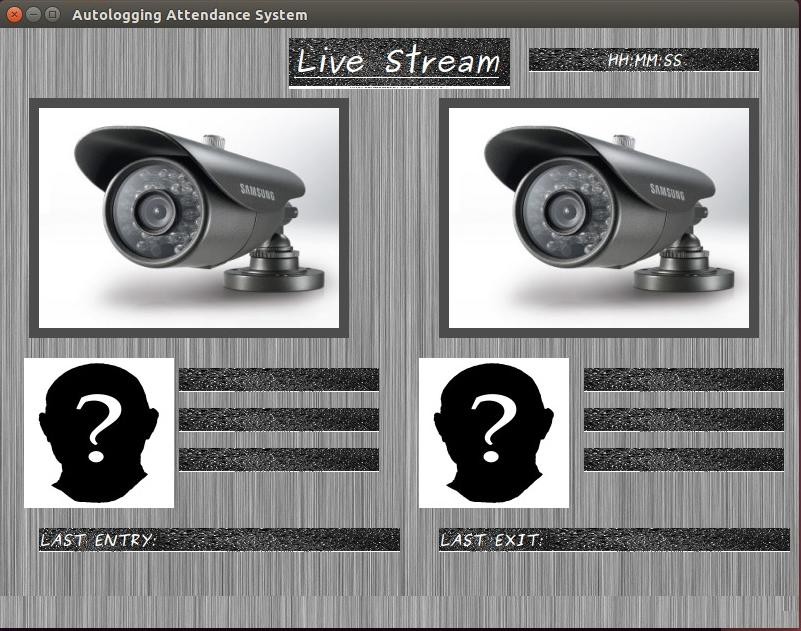
\includegraphics[width = 300pt]{guioapp}

\vspace{1cm}

\subsection{The System assembled}
The application creates three different recognizers, 
each recognizer trained on a different set of database. The database is divided into three sets based on the heights of the indivisiuals.
First set consists of indivisuals whose height is less than 125 cm. Second set consists of indivisuals whose height is between 125 and 135 
cm and the third set consists of indivisuals whose height is greater than 135 cm. The heights are as measured by the ultrasonic sensor.
\newline The Gui displays continuous video stream taken from the Entrance and Exit.
The stream is a live stream. The application runs face detection on the frames captured from the stream. If a face is detected, the
application requests the Arduino to send the height value via the serial terminal. 
Depending on the height reading returned by the arduino, the correspoding face recognizer is called and the detected face is given as
an input to that face recognizer. The image of the recognized person is displayed below the stream along with the name, entry/exit time 
and an ID. The same information is also logged in the excel workbook. This book consists of a sheet for each day, with the name of the 
sheet being the date.
\newline If an unknown person is recognized, then the image of the person is captured and stored in a separate folder along with 
the time stamp so that the authorized person can know about it later.
\newline The initial implementation was without the use of thread. In this case, the livestream was slow and somewhat non continuous. 
This is because the sequence of events were as follows:

\begin{itemize}
 \item Capture a frames
 \item Display it on the GUI
 \item Run the face detection algorithm on the frames
 \item If face is found, then run the face recognition algorithm on the detected face
 \item Capture the next frame and repeat the cycle
\end{itemize}

The processing between the capturing of two different frames took enough time to make the video look slow. So, threads were created 
to do the backend work, while in the front end, continuous frames were being captured and displayed. The sequence of events with the 
use of threads is as follows:

\begin{itemize}
 \item Capture a frame
 \item Display it on the screen
 \item If a thead is already running in the background, do not use this frame for processing and capture the next frame
 \item If there is no thread running in the background, create a thread and run the detection and recognition algorithm on 
  this frame in the background.
\end{itemize}

We maintained only a single thread at a time. Once the thread finished processing on the frame, then that thread died and the next
thread was created. You can maintain more than one thread to achieve speed but you will have to be careful about the global variables 
accessed by the threads. Proper data locking mechanisms should be used in that case to protect shared data.

\newpage
\section{Challanges faced}
\begin{enumerate}
 \item The database must be highly accurate and the expressions must be of same amenity for different person. Eg all the person
   must wink  their left or right eye only. Mixture of both will not be considered accurate.
 \item The training of the database involves lots of mathematics and deep understanding of wide variety of algorithms ranging
   from principal component analysis through machine learning upto neural networks and wavelet designs. Understanding algorithms 
   and deciding which one to use is a challenging task.
 \item The training of database involves training them through various layers called hidden layers with different weights. We trained
   upto 38 stages which took almost 7 to 8 hours. Still the accuracy was not as high as expected.
 \item The accuracy with just image processing was not as high as expected and the results were with some error. However this
   error was reduced greatly using height integration. It can be further reduced by integrating weight.
 \item Designing GUI from a wide range of available Python libraries was challenging since none of the library supported 
   direct video streaming. So we started saving images with 30fps and then reading them into the GUI. Thus using persistence of 
   vision concept to make those images being viewed as a continuous video.
\end{enumerate}

\newpage
\section{Future scope for improvements}
\begin{enumerate}
 \item We can add the data of newly joined employee in the database with the click of a button without having to make any changes
   in the code.
 \item An android app can be created so as to ensure all the employees to check whether their attendance is marked or not.
 \item We can even add an LCD display below the camera were a person can see his/her name or ID when detected and recognized.
 \item We can even make a sophisticated system where the door of the room automatically opens or closes on detection of the person, 
   making it smart room or smart office.
\end{enumerate}

\newpage
\section{Potential applications}
\begin{enumerate}
 \item As we said, this kind of Image processing for facial recognition can be used for auto logging attendance system in colleges. Since Our colleges have lectures of 1hr of which quarter time is wasted in taking attendance
 \item Not only in the case of human, this concept can be expanded to detect different objects and perform processing operations on them. For example, one can use this for auto car parking by detecting cars and classifying empty slots. This can even be used to find the traffic on the sides of highways or roads and clear them by giving larger waiting times to path with lesser commuters.
 \item The human face recognition system can be used at public places like railway stations to detect criminals and locate their path. This can be useful for surveillance  purpose.
\end{enumerate}

\newpage
\section{References}
\begin{itemize}
 \item Tutorial on face recognition by  Bikramjot Singh Hanzra
  \newline \textcolor{purple}{http://hanzratech.in/2015/02/03/face-recognition-using-opencv.html}
 \item Eigen faces
  \newline \textcolor{purple}{http://en.wikipedia.org/wiki/Eigenface}
 \item Principal Component Analysis
  \newline \textcolor{purple}{http://en.wikipedia.org/wiki/Principal\textunderscore component\textunderscore analysis}
 \item Eigen vectors
  \newline \textcolor{purple}{http://math.mit.edu/~gs/linearalgebra/ila0601.pdf}
 \item Yale Face Database
  \newline \textcolor{purple}{http://vision.ucsd.edu/content/yale-face-database}
 \item Getting started with Arduino
  \newline \textcolor{purple}{https://www.arduino.cc/en/Guide/HomePage}
\end{itemize}


\end{document}